\begin{figure}[htbp]
    \centering
    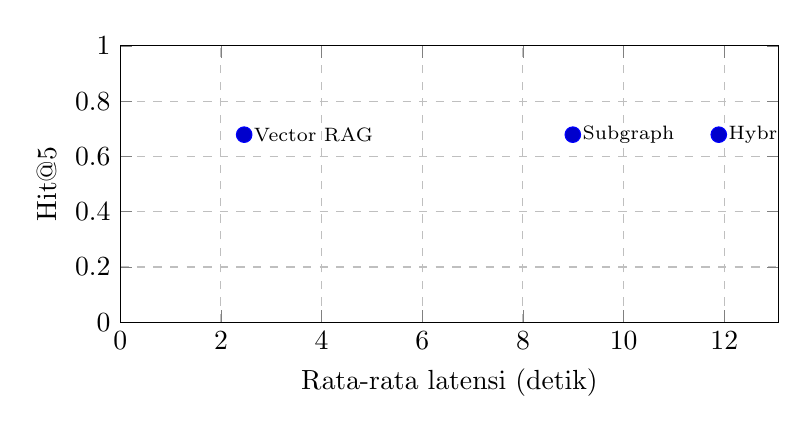
\begin{tikzpicture}
    \begin{axis}[
        width=0.82\textwidth,
        height=0.42\textwidth,
        xlabel={Rata-rata latensi (detik)},
        ylabel={Hit@5},
        ymin=0, ymax=1.0,
        xmin=0,
        ymajorgrids=true,
        xmajorgrids=true,
        grid style=dashed,
    ]
        \addplot+[only marks, mark=*, mark size=2.8pt] coordinates {(2.4620,0.6786) (8.9910,0.6786) (11.8910,0.6786)};
        \node[font=\scriptsize, anchor=west] at (axis cs:2.4620,0.6786) {Vector RAG};
        \node[font=\scriptsize, anchor=west] at (axis cs:8.9910,0.6786) {Subgraph};
        \node[font=\scriptsize, anchor=west] at (axis cs:11.8910,0.6786) {Hybrid};
    \end{axis}
    \end{tikzpicture}
    \caption{Trade-off antara latensi dan Hit@5 pada mode retrieval}
    \label{fig:bab4-eval-latency-hit}
\end{figure}
